\RequirePackage{pdfmanagement-testphase}
\DeclareDocumentMetadata{}
\documentclass[letterpaper,openany,twoside,twocolumn]{book}

\newcommand{\PATH}{../../../../../}

\usepackage[justified]{\PATH dndtemplate/dnd}

\usepackage{\PATH regions/stylesheets/regions_stylesheet}
\usepackage{\PATH regions/stylesheets/dungeon_stylesheet}
\usepackage{\PATH regions/stylesheets/shadowfy}

\usepackage[english]{babel}
\usepackage[utf8]{inputenc}

%\newcommand{\entryfont}{\DndFontStatBlockBody}
\newfontfamily\entryfont{Kalam}[Path=\PATH template/fonts/,Extension=.ttf,UprightFont=Kalam-Regular,BoldFont=Kalam-Bold]
\newfontfamily\titlefont{Modesto Bold(2)}[Path=\PATH template/fonts/,Extension=.otf,UprightFont=Modesto Bold(2),BoldFont=Modesto Bold(2)] % requires XeLaTeX or LuaTeX
\newfontfamily\notefont{Copenhagen}[Path=\PATH template/fonts/,Extension=.ttf,UprightFont=Copenhagen, BoldFont=Copenhagen] % requires XeLaTeX or LuaTeX

\begin{document}
	\graphicspath{{./images},{./monsters/Blank_Monster/images}}

\DungeonSheetGeometry

\dungeonTitlePage{MarzDarkRed/white}%
	{0cm}%
	{-0.25cm}%
	{height=\paperheight}%
	{Tomb_of_the_Scorpion_King_filter.png}%
	{%
		{TomboftheScorpionKing1}{Page \thepage}{Art}{https://www.imagine.art/}{Tomb of the Scorpion King}{ImagineAI}%
	}%
	{Tomb of the Scorpion King}%
	{black/white}%
	
\clearpage
\section*{History}

\clearpage

\twocolumn[\section*{Tomb of the Scorpion King - Entrance Area}
\centerline{\begin{minipage}{\paperwidth}
\begin{tikzpicture}[outer sep=0pt, inner sep=0pt, every shadow/.style={opacity=.8,fill=black}]
	\node {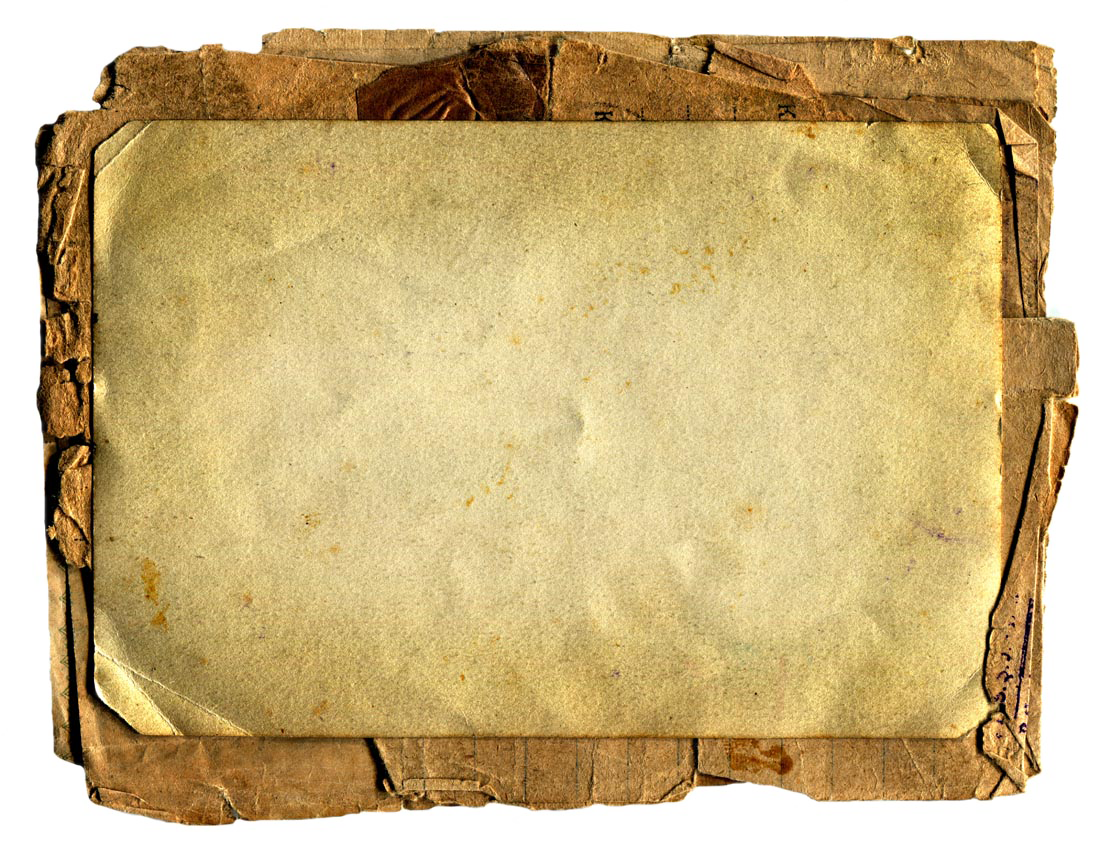
\includegraphics[width=\paperwidth - 8pt, height=14cm]{\PATH regions/stylesheets/images/backgrounds/Dungeons/dungeon_map.png}};
	
	% Guidelines
	\begin{scope}[scale=0.3, every path/.style={black!80, thick}]
		\foreach \y in {0,...,28}
			\draw (-26, -14 + \y) -- ++(52, 0);
		\foreach \x in {0,...,52}
			\draw (-26 + \x, -14) -- ++(0, 28);
	\end{scope}
	
	\begin{scope}[scale=0.3]
		\path[clip, rounded corners=0.5cm] (-1.67\paperwidth + 250pt, -15) rectangle (1.67\paperwidth - 250pt, 15);
		
		\node[inner sep=0pt,outer sep=0pt,clip,rounded corners=0.5cm] {{\transparent{0.7}
\includegraphics[width=\paperwidth-150pt, height=9cm]{\PATH regions/stylesheets/images/backgrounds/Dungeons/sand_dungeon_texture.jpg}}};
		
		% Assets below Shadows
		\begin{scope}
			% Contour Lines			
			\path[draw] (-4,2) -- ++(0,-5) arc[start angle=-180, end angle=0, radius=3] -- ++(0,5);
			\path[draw] (-4.5,2) -- ++(0,-5) arc[start angle=-180, end angle=0, radius=3.5] -- ++(0,5);
			\path[draw] (-5,3) -- ++(0,-6) arc[start angle=-180, end angle=0, radius=4] -- ++(0,6);
			\path[draw] (-5.5,4) -- ++(0,-7) arc[start angle=-180, end angle=0, radius=4.5] -- ++(0,7);
			\path[draw] (-6,4) -- ++(0,-7) arc[start angle=-180, end angle=0, radius=5] -- ++(0,7);
			\path[draw] (-6.5,4) -- ++(0,-7) arc[start angle=-180, end angle=0, radius=5.5] -- ++(0,7);
			\path[draw] (-7,4) -- ++(0,-7) arc[start angle=-180, end angle=0, radius=6] -- ++(0,7);
			
			% Images
			\node[inner sep=0pt,outer sep=0pt, rotate=180] at (-1,-2.5) {
\includegraphics[height=1.5cm]{Scorpion_Golden_Statue.png}};
			\node[inner sep=0pt,outer sep=0pt, yscale=-1, rotate=-10] at (-6.5,-1.5) {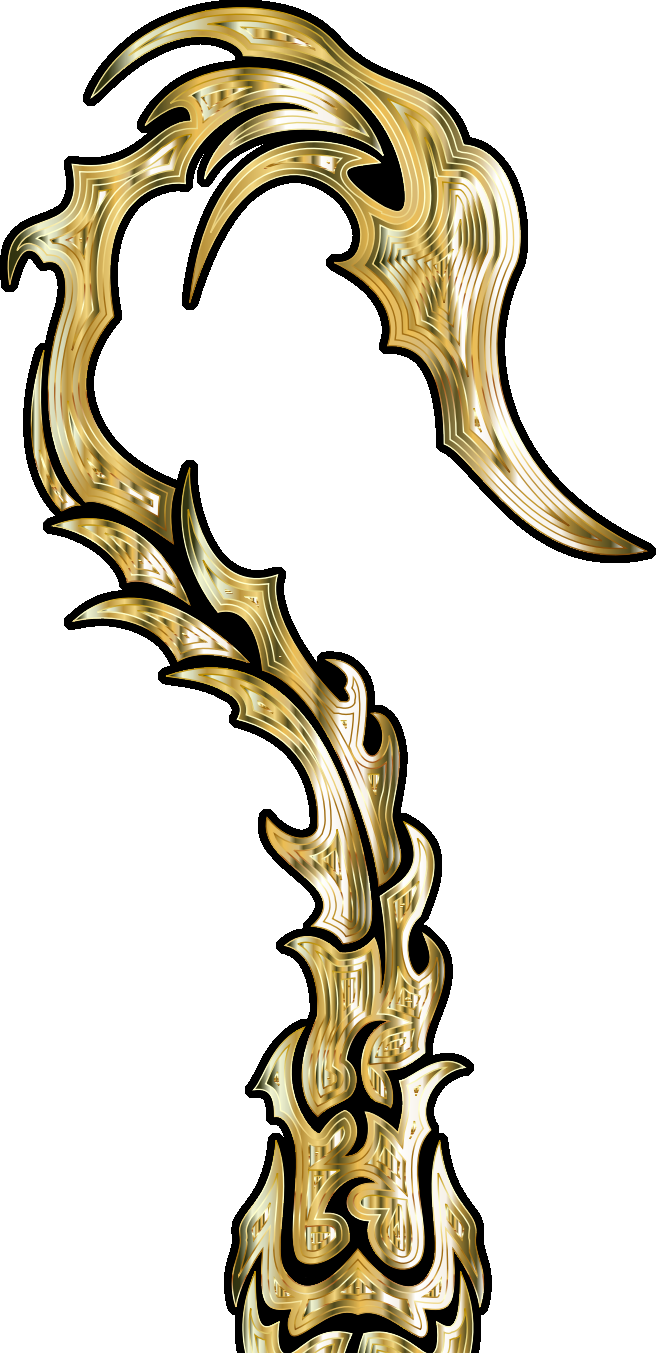
\includegraphics[height=3.6cm]{Scorpion_Golden_Ornament_Tail.png}};
			\node[inner sep=0pt,outer sep=0pt, scale=-1, rotate=-10] at (4.5,-1.5) {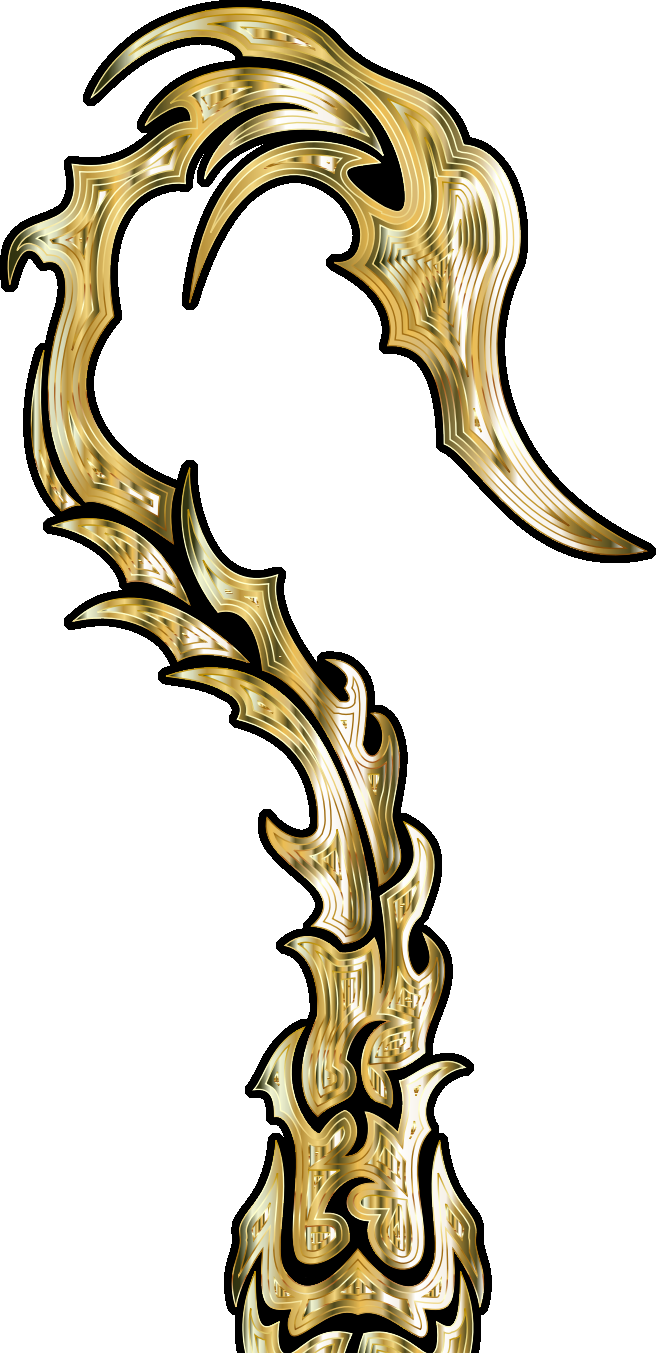
\includegraphics[height=3.6cm]{Scorpion_Golden_Ornament_Tail.png}};
		
			% Traps
			\trapField{8,4}
			\trapField{9,4}
			\trapField{9,5}
			\trapField{8,6}
			\trapField{10,7}
			\trapField{9,8}
			\trapField{10,8}
			\trapField{10,9}
			
			%Stairs
			\stairsField{sand}{13,8}{anchor=south west}{0.3cm}{0.3cm}
			%\stairsField{sandspiral}{-12,9}{rotate=0, yscale=-1}{0.6cm}{0.6cm}
			
			% Chests
			\chestField{red}{closed}{8,10}{anchor=south west}{0.3cm}{0.3cm}
			\chestField{red}{closed}{9,10}{anchor=south west}{0.3cm}{0.3cm}
		\end{scope}
		
		\path[clip, drop shadow] (-28,-16)
		-- ++(15,0) -- ++(0,25) arc[start angle=180, end angle=90, radius=1] -- ++(2,0) -- ++(0,-6) arc[start angle=-180, end angle=0, radius=1] arc[start angle=90, end angle=15, radius=4] -- ++(6.275,0) arc[start angle=-195, end angle=-270, radius=4] -- ++(2,0) -- ++(0,7) -- ++(2,0) -- ++(0,-1) -- ++(1,0) -- ++(0,3) -- ++(3,0) -- ++(0,-5) -- ++(-1,0) -- ++(0,4) -- ++(-1,0) -- ++(0,-3) -- ++(-1,0) -- ++(0,-21) -- ++(-24,0) -- ++(0,-5)
		-- (28,-16) -- (28,16) -- (-28,16) -- cycle;
		
		\node[inner sep=0pt,outer sep=0pt,clip,rounded corners=0.5cm] at (0,0) {{\transparent{0.7}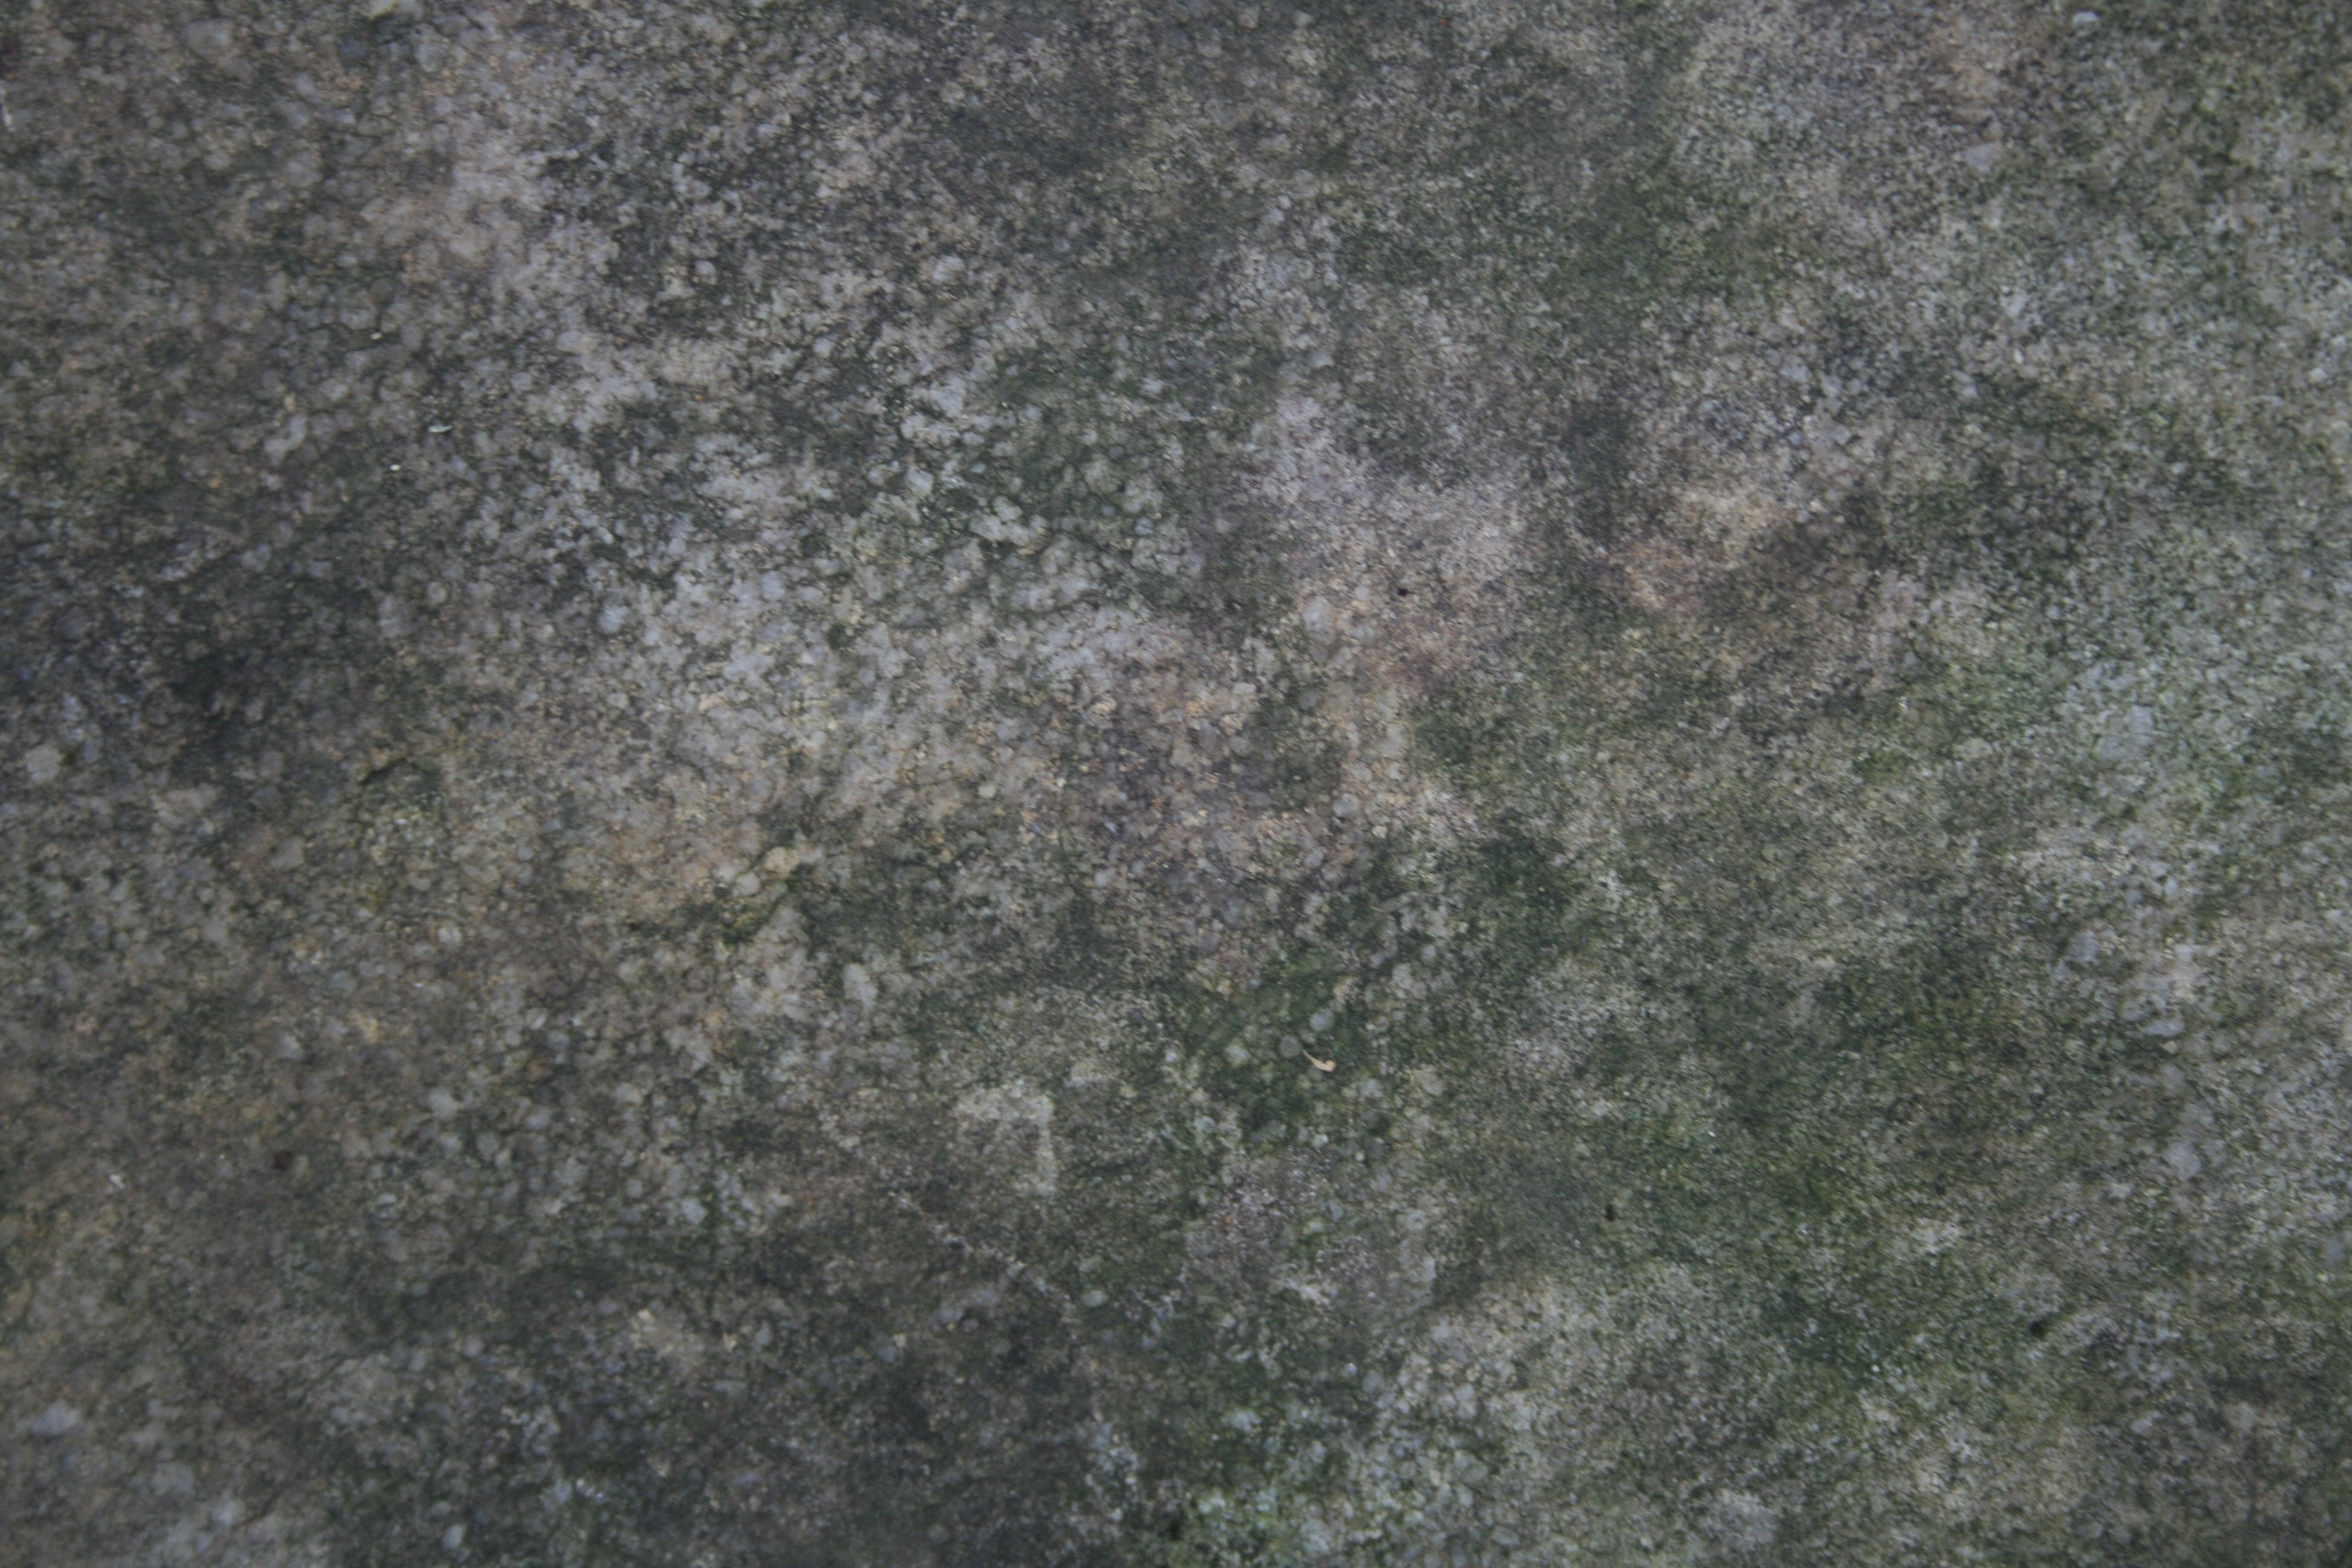
\includegraphics[width=\paperwidth-150pt, height=9cm]{\PATH regions/stylesheets/images/backgrounds/Dungeons/rocky_dungeon_texture.jpg}}};
		
		\path[clip, drop shadow] (-28,-16)
		-- ++(15,0) -- ++(0,5) -- ++(11,12) -- ++(0,2) -- ++(-2,0) -- ++(0,6) -- ++(6,0) -- ++(0,-6) -- ++(-2,0) -- ++(0,-2) -- ++(11,-12) -- ++(0,-5) 
		-- (28,-16) -- (28,16) -- (-28,16) -- cycle;
		
		\node[inner sep=0pt,outer sep=0pt,clip,rounded corners=0.5cm] at (0,0) {\includegraphics[width=\paperwidth-150pt, height=9cm]{\PATH regions/stylesheets/images/backgrounds/Dungeons/sandstone_dungeon_texture.jpg}};		
	\end{scope}
	
	% Assets above Shadows
	\begin{scope}[scale=0.3]
		% Doors
		\doorField{secret}{(11,9.5)}{west}{0}{0.1cm}{0.3cm}
		\doorField{doublewood}{(-1,0.5)}{south}{0}{0.61cm}{0.3cm}
		
		% Stairs
		\stairsField{sandspiral}{-12.04,9}{rotate=0, yscale=-1}{0.6cm}{0.6cm}
		
		% Numbers
		\indicatorNumberField{(-1,-3)}
		\indicatorNumberField{(-5,-5)}
		\indicatorNumberField{(-2.5,1)}
		\indicatorNumberField{(1,-10)}
		\indicatorNumberField{(9.5,7)}
		\indicatorNumberField{(11.5,8.5)}
		\indicatorNumberField{(9,11)}
		\indicatorNumberField{(-12.5,8.5)}
	\end{scope}
	
	% Outer Ornaments
	\begin{scope}
		\node[inner sep=0pt,outer sep=0pt, xshift=-0.5\paperwidth+135.5pt] {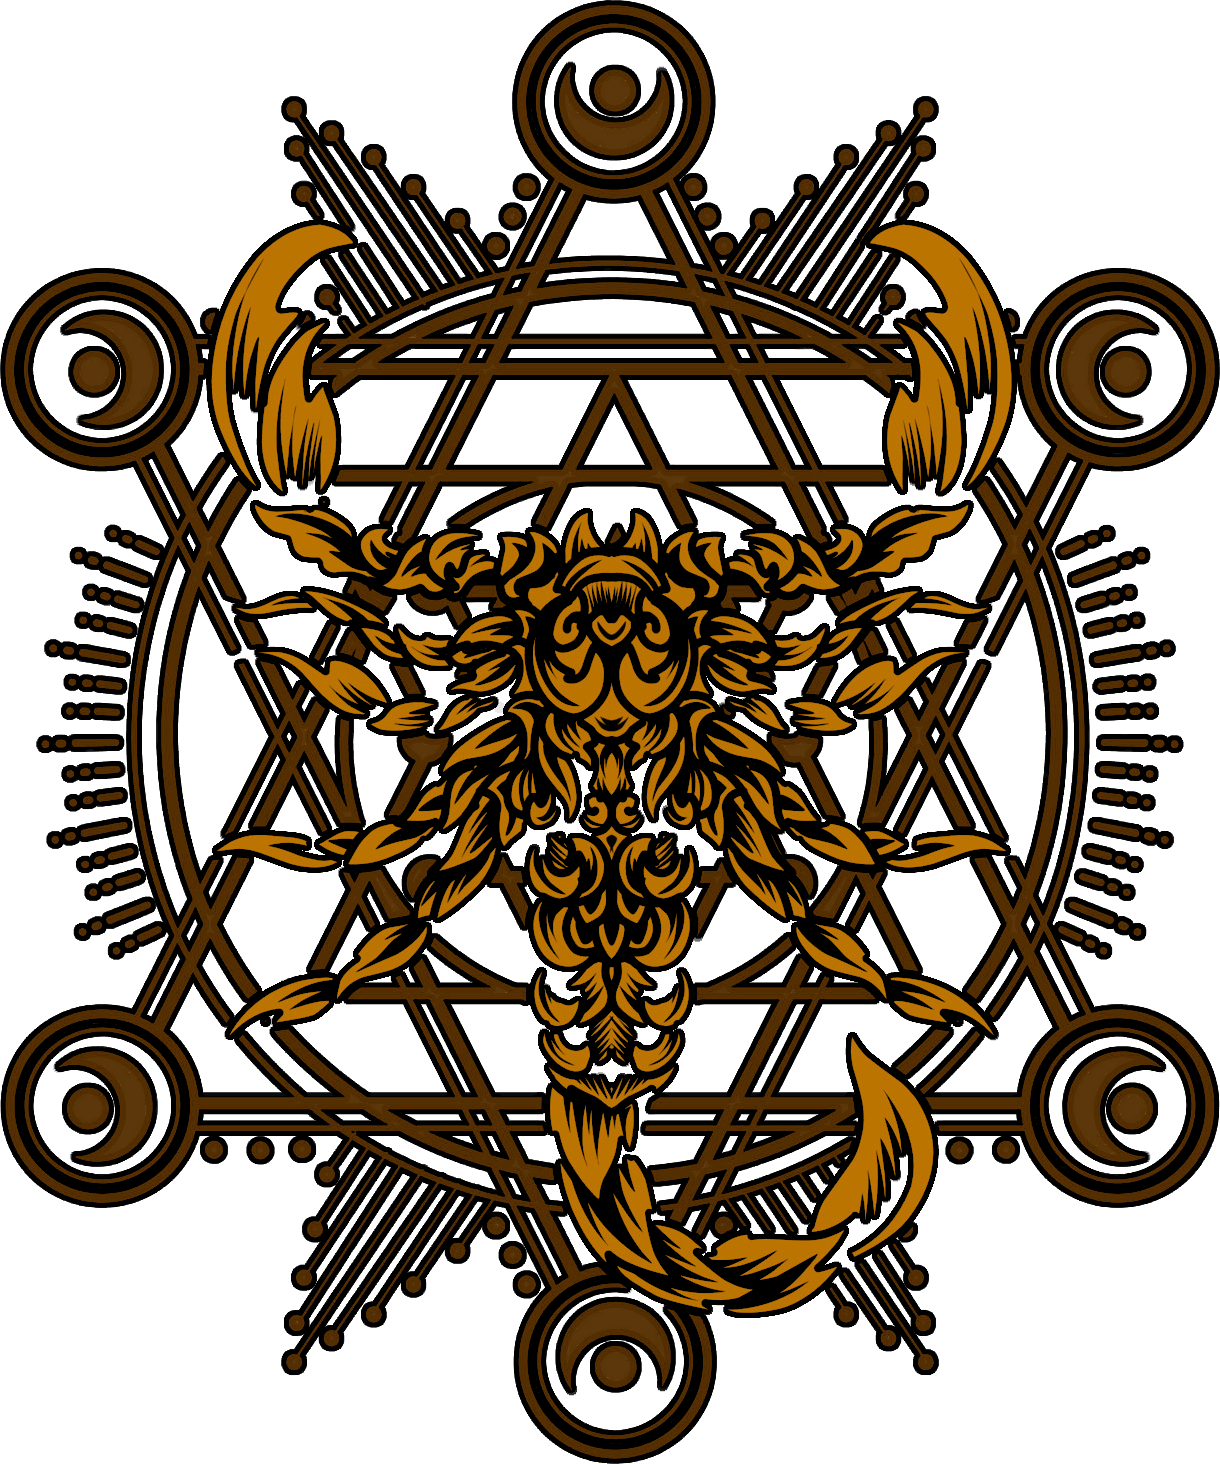
\includegraphics[height=4.5cm]{Scorpion_Ornament_Banner.png}};
		\node[inner sep=0pt,outer sep=0pt, xshift=0.5\paperwidth-145pt, xscale=-1] {
\includegraphics[height=6cm]{Scorpion_Colorful_Ornament.png}};
	\end{scope}
\end{tikzpicture}
\end{minipage}}]

\subsection*{1. Golden Scorpion Statue}
{\entryfont
	Before the imposing entrance to the "Tomb of the Scorpion King" stands a meticulously crafted golden scorpion statue. It is raised upon a pedestal, its intricate design capturing the essence of the desert's most fearsome predator.
	
	\textbf{Puzzle} Its right eye socket is adorned by a orange gemstone (worth 500 GP) whereas the left eye socket remains empty.\\
	When the gemstone is removed from the right eye socket four Giant Scorpions appear from the ground surrounding the entrance area attacking the adventurers. One of these drops a particular \textbf{Silver Scorpion Stinger Key}.\\
	The placement of different gems into either socket can have different, repeatable effects:
	\begin{itemize}
		\item \textbf{Violet Eye Gemstone}\\ If the orange and the violet gemstones are placed into the eye sockets the main entrance opens.
		\item \textbf{Blue Eye Gemstone}\\A chain lightning emerges from the scorpion statue's eyes hitting the nearest character. Two bolts then leap from that target to as many as two other targets, each of which must be within 20 feet of the first target A target must make a DC 17 Dexterity saving throw. The target takes \DndDice{4d8} lightning damage on a failed save, or half as much damage on a successful one.
		\vfill\eject
		\item \textbf{Red Eye Gemstone}\\
		The statue produces extreme heat around it. Each creature within 10 feat of it must make a DC 18 Constitution saving throw taking \DndDice{1d6} fire damage and gaining one level of exhaustion on a failed save. This saving throw must be repeated after 1 hour when still standing near the statue.
		\item \textbf{Common Gemstone}\\
		A swarm of scorpions (see statblock) emerges from the statue's torso attacking the player that placed the gem into the socket.
	\end{itemize}
}

\subsection*{2. Golden Scorpion Ornaments}
{\entryfont
	Winding their way up the stairs these scorpion tails ornaments are in no way inferior in craftmanship. Their intricate curvature imparts an aura of dynamic movement, as if the tails are poised to lash out at any who dare to disturb their path. These statues are more than mere decorations - they hold a magical secret.
	
	Upon closer inspection, you notice a faint, iridescent shimmer playing upon the surface of the tails. These enchantments grant the tails a unique and perilous quality. If touched, one of the following effects are triggered, initiating a response that promises challenge.
	\clearpage
	\begin{itemize}
		\item On a failed DC 15 Constitution saving throw the character is poisoned for 1d4 minutes.
		\item An illusionary Giant Scorpion appears. It cannot be interacted with and disappears after 1d6 minutes.
		\item A sudden cascade of sand swirls up from the ground. Each character within 5 feet must succeed a DC 15 Constitution saving throw or is blinded for 1 minute.
	\end{itemize}
}

\subsection*{3. Main Entrance Door}
{\entryfont
	Crafted from massive timbers of weathered wood, the entrance exudes a sense of both strength and antiquity. The grandeur of the temple is mirrored in the sheer scale of the entrance, which dwarfs those who approach it.
	
	It can only be opened by solving the Golden Scorpion Statue Puzzle and not by other non-magical means.
}

\subsection*{4. Buried Eye Gemstone}
{\entryfont
	A subtle 'X' is etched into the ground, a quiet testament to hidden treasure. For those with a keen eye (DC 15 Perception Check), its presence hints at the location of a small, buried strongbox, patiently awaiting discovery. Unearthing the prize demands dedication, a ten-minute endeavor that unveils the secrets held within, but the process is expedited to a mere minute when a shovel joins the effort. Inside the strongbox, a single gem gleams - an enigmatic \textbf{Red Eye Gemstone}.
}

\subsection*{5. Traps in right Passage}
{\entryfont
	Based on the location of the trap there are 3 different kinds placed in the right passageway:
	\begin{itemize}
		\item \textbf{In front of the secret door}\\
		Thunderwave Trap (DEX DC 18) that knocks a character back 20 feet. On an additional failed Consitution saving throw (DC 16) the target also takes \DndDice{1d6} force and \DndDice{1d8} bludgeoning damage.
		\item \textbf{Near the cliffside on both sides}\\
		Stron Drop Trap (DEX DC 14) that deals \DndDice{2d10} bludgeoning damage on a failed save.
		\item \textbf{Middle of passageway}\\
		Poisoned Spring Trap (DEX DC 16) that deals \DndDice{1d8} piercing damage on a failed save. On an additional failed Consitution saving throw (DC 18) the target is poisoned.
	\end{itemize}
}

\subsection*{6. Secret Door}
{\entryfont
	Embedded within the canyon's cliffside lies a covert passage, concealed by artful design. With a perceptive touch (DC 18 Perception or Investigation Check), the discerning eye may trace the subtle contour of a stone door, masterfully blended into the rugged façade. An engraving, reminiscent of a scorpion's stinger, graces this concealed entryway, a whispered promise of the secrets that lie beyond. Unveiling the portal's mystery requires the touch of destiny - a \textbf{Silver Scorpion Stinger Key}, a key to fate itself, snugly placed within the waiting notch.
}

\subsection*{7. Twin-Chests}
{\entryfont
	Nestled at the conclusion of the rightward path, a dual set of chests emerges, twin entities united in their enigma, virtually indistinguishable from one another. Side by side, they stand as a testament to the balance of secrets they guard.
	
	\vfill\eject
	
	\textbf{Treasure}
	In one of the chests the following treasures can be found:
	\begin{itemize}
		\item \textbf{Blue Eye Gemstone}
		\item 1d4 Potion of Cure Poison
		\item Shovel
		\item a Shield
	\end{itemize}
	
	\textbf{Trapped Treasure}
	The other chest is a transformed mimic that will attack the character that interacts or investigates it. When the mimic is killed the following note can be found within it:\\\\
	\begin{tikzpicture}
		\NoteMessage{\linewidth}{18}{note_parchment_background_vertical.png}{%
			2E 214 17th of Alturiak\\
			I recall the words:
			\begin{center}
				The first bathes in the fading sun's light,\\
				Its beauty a beacon through the dusky night.\\
				The second mirrors dawn's tender embrace,\\
				A promise of warmth in the morning's grace.\\
			\end{center}
			Placing the orange gem in the socket, I wait, but nothing happens. Relief washes over me as the surroundings remain still. The riddle's guidance rings true.\\\\
			But my hand hesitates as it hovers over the red gem. The allure is undeniable. It seems to thrum with warmth and energy. As I gingerly place it in the socket, a sudden rush of heat washes over me, an intense warmth that makes me reel back.\\\\
			The entrance still remains closed, maybe I find something else . . .
		}%
	\end{tikzpicture}
	\hfill\\
	Furthermore the following items can also be found in the dead mimic's corpse:
	\begin{itemize}
		\item 1d6 Potion of Cure Poison
		\item 200 GP
		\item Potion of Greater Healing
		\item an Amethyst (200 GP)
	\end{itemize}
}

\subsection*{8. Staircase to Scorpion's Gaze}
{\entryfont
	Ascending from the depths of the canyon, a round sandstone staircase spirals upwards, its form a testament to the passage of countless ages. Carved with both precision and the artistry of time's touch, the staircase clings to the canyon walls with weathered grace. Each step, worn smooth by the footfalls of generations, tells a tale of pilgrimage and discovery.
	
	The staircase leads to a lookout point, perched high above the entrance. Here, a plateau of the canyon extends, a sanctuary that time forgot. The vista before you is breathtaking, a canvas painted with the hues of desert life. The plateau's edge offers a vantage point that seems to touch the very heavens, granting you a commanding view of the canyon's expanse and the hidden entrance below.
}

\DungeonBannerGraphic{Scorpion's Gaze}{12.25cm}{13.5cm}{Scorpion_s_Gaze.png}{}
{\entryfont
	Upon reaching the pinnacle of the ancient sandstone staircase, the world stretches out before you in all its splendor. The lookout point, perched high above the expansive canyon plateau, revealing the sprawling grandeur of the canyon plateau in vivid detail. The rugged terrain, an untamed canvas of sun-kissed earth and wind-carved rock, extends as far as the eye can see. The landscape is alive with the hues of the desert, its palette ranging from warm ochres to deep russets, illuminated by the sun's golden embrace.
	
	The central figure is a resplendent scorpion, its stinger poised as if to strike the very heavens. Its body, carved with meticulous detail, forms the foundation for the grand design. Ingeniously, stairs are engraved into the scorpion's segmented back, leading to a small lookout platform nestled high above the ground. From here, a breathtaking panorama unfolds, revealing the canyon's undulating topography.
	
	Emerging underneath the scorpion's figure, a substantial circular ring evokes the sinuous form of a centipede's body. This ring forms a courtyard of reverence before the statue. As you step onto its well-worn surface, you find yourself surrounded by an aura of ancient whispers, as if the stones themselves bear the memory of those who came before.
	
	A narrow bridge, adorned with scorpion-themed ornaments that glisten in the sunlight, spans the circular ring's expanse. Its path guides you across the symbolic embrace of the centipede ring and ushers you into the courtyard plaza before the great scorpion statue. Here, amid a harmonious convergence of artistry and nature, you stand witness to a sacred meeting of the past and the present.
}

\vfill\eject\hfill\\\vspace*{0.5\fontdimen6\font}
\subsection*{Mysteries and Dangers}
{\entryfont
	Amid the beauty and grandeur of the lookout point, mysteries entwine with potential perils, weaving a tale of challenge and discovery. Upon the lofty viewing platform, a pedestal sits adorned with a single Violet Eye Gemstone. Its presence hints at an unspoken role, a piece in the puzzle of the plateau's enigma.
	
	The gem's allure is undeniable, and a curious hand plucking it from its resting place triggers an audible click that reverberates through the air. A sudden realization dawns as the bridge leading back out the courtyard, a pathway that appeared a moment ago inviting and open, rises with a mechanical precision. A shiver races down spines as the once-accessible escape route becomes a cruel cage, ensnaring all within the courtyard's boundaries.
	
	As tension thickens, a chorus of roars and growls pierces the air. From shadowed crevices and hidden corners emerges a Manticore, accompanied by \DndDice{1d4} Giant Scarabs. Its intentions shrouded in malice, the monster embodies the very essence of danger that lurks within the tomb. A battle unfolds, and the clash of steel and the echoes of spells become a dance of survival against the backdrop of the plateau's commanding vista.
	
	 As the Manticore succumbs to defeat, the bridge descends once more, its mechanisms relenting. Freedom beckons, a reward for the valor displayed. The adventurers stand amidst the aftermath, surrounded by the cryptic aura of the lookout point, a place where triumph and trepidation mingled.
}
\end{document}